\chapter{HIỆN THỰC HỆ THỐNG PHÁT HIỆN TIN NÓNG}
\ifpdf
    \graphicspath{{Chapter3/Chapter3Figs/PNG/}{Chapter3/Chapter3Figs/PDF/}{Chapter3/Chapter3Figs/}}
\else
    \graphicspath{{Chapter3/Chapter3Figs/EPS/}{Chapter3/Chapter3Figs/}}
\fi

\section{Mở đầu}
Chương này sẽ trình bày về thiết kế, chi tiết cài đặt, các thư viện và framework được sử dụng để xây dựng hệ thống lọc rác tin tức.

\section{Mô hình hệ thống}
Dưới đây là mô hình của các thành phần chính hệ thống:
\begin{figure}[H]
	\centering
	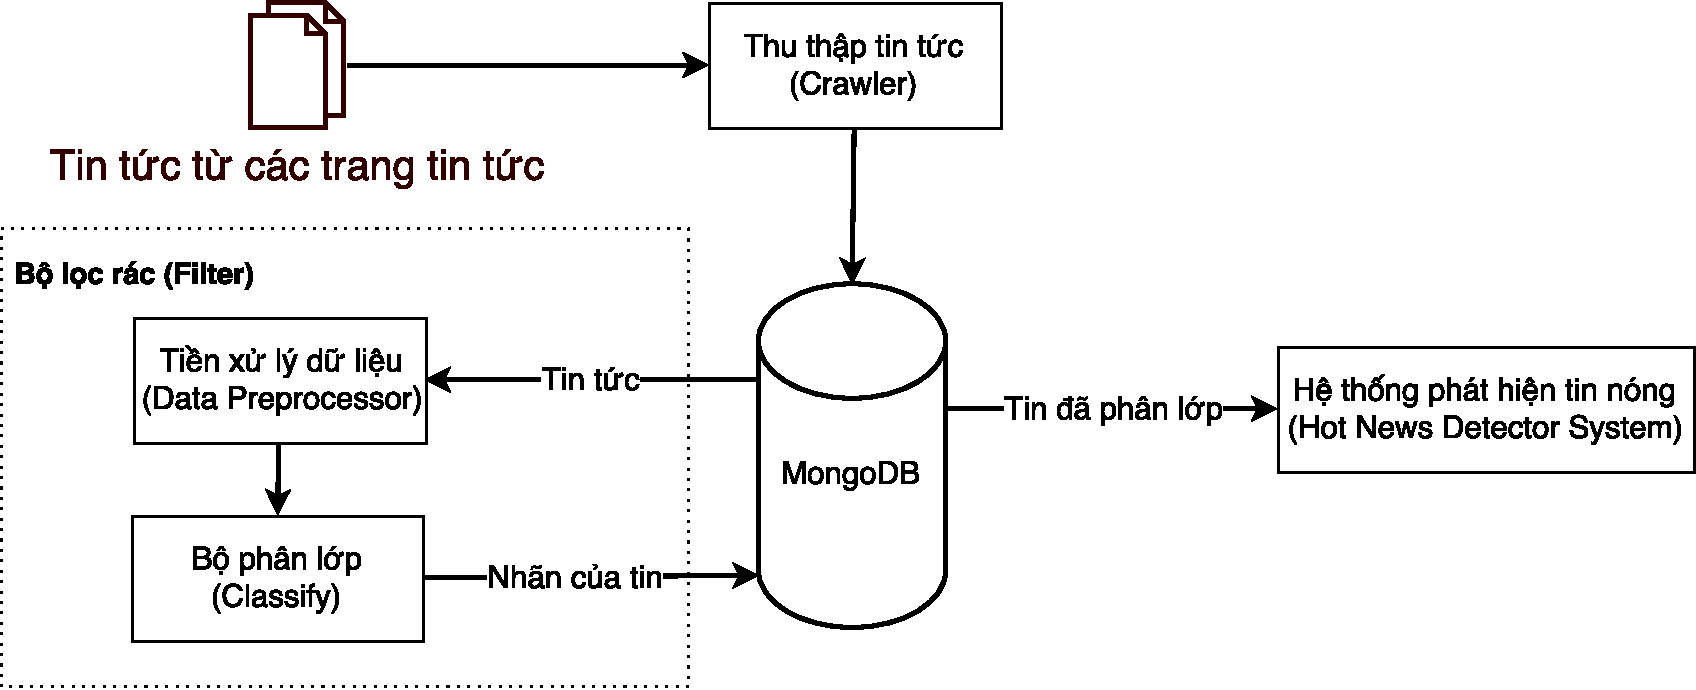
\includegraphics[width=0.9\linewidth]{Chapter3/Chapter3Figs/PDF/SystemArchitecture}
	\caption{Các thành phần chính của hệ thống}
	\label{fig:systemarchitecture}
\end{figure}
\subsection{Luồng xử lý dữ liệu}
	Hệ thống phân loại tin tức được chia thành 2 hệ thống nhỏ hơn, đó là hệ thống Crawler và hệ thống Spam Filtering: 
	\begin{itemize}
		\item Hệ thống Crawler có nhiệm vụ đồng bộ hóa tin tức đã được lấy về từ các trang tin tức và thực hiện tiến trình phân lớp(classification process) cho các tin tức đó.
		\item Hệ thống Spam Filtering cung cấp các API: phân loại tin tức bằng tiêu đề hoặc bằng URL của tin đó, cung cấp dữ liệu thống kê cho các tin đã phân lớp ở hệ thống Crawler, API feedback khi các tin dự đoán sai mong muốn của bình luận viên.
	\end{itemize}
Hệ thống Crawler phục vụ cho bài toán Hot News Detection, sau khi tin tức được lọc rác, các tin tức được đánh giá là rác sẽ bị bỏ qua khi đưa vào hệ thống Hot News Detection.
Hệ thống Spam Filtering chủ yếu phục vụ cho biên tập viên. Biên tập viên sử dụng hệ thống thông qua giao diện Spam Filtering để sử dụng chức năng phân lớp tin tức hoặc xem các số liệu thống kê về tin tức đã phân lớp lưu trong cơ sở dữ liệu.
\section{Tiến trình phân lớp}
\begin{figure}[H]
	\centering
	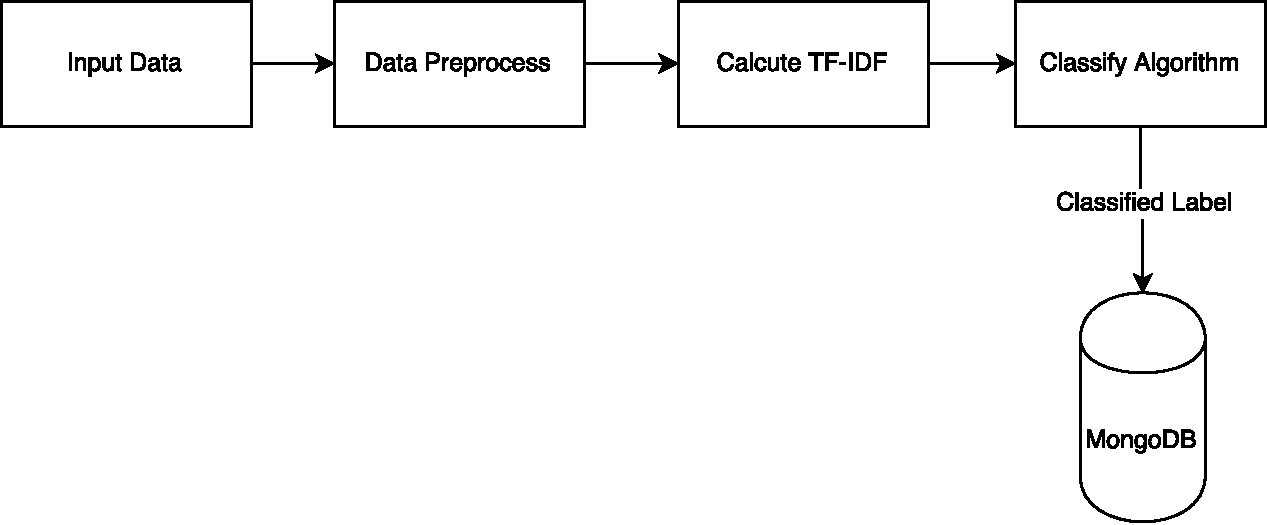
\includegraphics[width=0.9\linewidth]{Chapter3/Chapter3Figs/PDF/ClassifyProcess}
	\caption{Tiến trình phân lớp}
	\label{fig:classifyprocess}
\end{figure}
Tiến trình phân lớp sẽ bao gồm \nameref{sec:DataPreprocessor} và phân hệ Classify.
Phân hệ Classify bao gồm: \nameref{sec:newsClassify} và \nameref{sec:spamCategory}.
Luồng xử lý của tiến trình phân lớp sẽ thực thi theo hình \ref{fig:classifyprocess} :
\begin{itemize}
	\item Input data: Dữ liệu đầu vào, gồm các document bao gồm Id và title của tin được lưu dưới định dạng csv. Mỗi dòng trong file csv bao gồm 2 cột: Id và title của tin tức đó.
	\item Data Preprocess: Dữ liệu ở cột title  sẽ thực thi theo \refname{sec:DataPreprocessor}. Output của quá trình này là file csv với cột title đã được xử lý.
	\item Calculate TF-IDF: Dữ liệu title sau khi được tiền xử lý sẽ được tính TF-IDF. Output của quá trình tính tf-idf sẽ là file csv chứa các kết quả tf-idf theo attribute của tập từ điển.
	\item Classify Algorithm: Hệ thống sẽ sử dụng thư viện Weka để phân lớp dữ liệu. Output của quá trình này sẽ là nhãn(Label) của tin. Sau đó, nhãn sẽ được lưu xuống cơ sở dữ liệu MongoDB.
\end{itemize}

\section{Phân hệ thu thập dữ liệu (Data Streaming)} \label{sec:DataStreaming}
Module này sử dụng hệ thống Crawler để lấy các bài đăng từ nhiều nguồn tin tức lưu trữ ở cơ sở dữ liệu MySQL và đưa qua cơ sở dữ liệu MongoDB, hệ thống sẽ thực hiện các chức năng:
	\begin{itemize}
		\item Connect vào cơ sở dữ liệu mySQL để lấy các bài bài báo.
		\item Xóa các bài viết trùng.
		\item Lưu trữ xuống cơ sở dữ liệu MongoDB
	\end{itemize}
\section{Phân hệ tiền xử lý dữ liệu (Data Preprocessor)}
\label{sec:DataPreprocessor}
Module tiền xử lý có nhiệm vụ chính gồm loại bỏ URL, thực hiện tách từ, loại bỏ stopwords và biểu diễn dữ liệu thành vector trọng số tf-idf. Trước khi chạy thuật toán phân loại, dữ liệu được lấy ra từ MongoDB và tiền xử lý phần nội dung của bài báo bằng các bước sau:
	\begin{enumerate}
		\item Loại bỏ URL bằng regular expression.
		\item Tách từ sử dụng thư viện TPSegmenter. Bước này dùng để biểu diễn các từ ghép trong tiếng Việt bằng cách thêm gạch nối giữa các tiếng của từ.\\
		Ví dụ: \textit{"Vụ tai nạn 13 người chết: Đã giám định mẫu máu tài xế xe tải"} qua bộ tách từ sẽ thành \textit{"Vụ tai\_nạn 13 người chết : Đã giám\_định mẫu máu tài\_xế xe\_tải"}.
		\item Loại bỏ các từ trong danh sách gồm 813 stopwords.
		\item Tính và biểu diễn dữ liệu thành vector tf-idf và metadata.
	\end{enumerate}

\section{Phân hệ phân loại tin tức}
\label{sec:newsClassify}
Sử dụng model đã train trước đó để phân loại tin tức. Model sử dụng thuật toán SVM đã trình bày ở chương 2 làm thuật toán chính để phân loại tin tức. Hiện tại hệ thống có 2 nhãn đã được định nghĩa trước đó:
	\begin{itemize}
		\item \textit Không rác
		\item \textit Rác
	\end{itemize}

Sau khi đã phân loại, hệ thống sẽ lưu nhãn đã gán cho tin tức xuống cơ sở dữ liệu MongoDB.

\section{Phân hệ phân loại loại rác}
\label{sec:spamCategory}
Hệ thống sẽ lấy những tin được gán nhãn "Rác" ở bước phân loại tin tức ở trên để phân loại loại rác cho tin đó. Hiện tại có 3 loại rác đã được định nghĩa trước:
\begin{itemize}
	\item \textit Quảng cáo
	\item \textit Tuyển dụng
	\item \textit Chia sẻ
\end{itemize}

\section{Thiết kế hệ thống} 
	\begin{figure}[H]
		\centering
		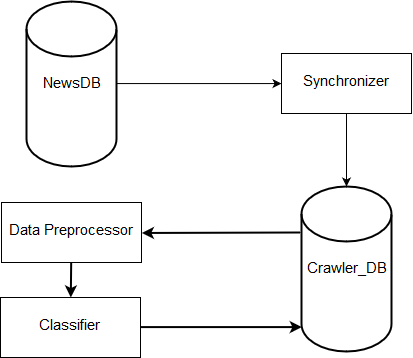
\includegraphics[width=0.5\linewidth]{Chapter3/Chapter3Figs/CrawlerSystem}
		\caption{Kiến trúc hệ thống crawler tin tức}
		\label{fig:crawlersystem}
	\end{figure}
Hệ thống Crawler được xây dựng độc lập bao gồm phân hệ thu thập dữ liệu, phân hệ tiền xử lý và phân hệ phân lớp để chạy ngầm nhằm thu thập và phân loại thông tin
	\begin{figure}[H]
		\centering
		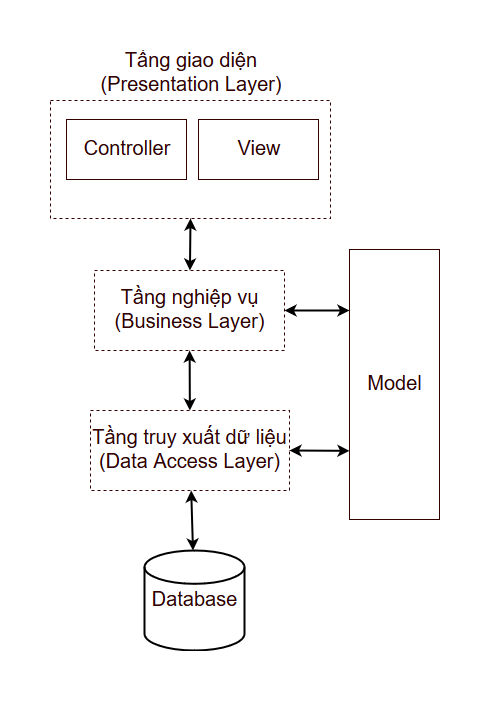
\includegraphics[width=0.5\linewidth]{Chapter3/Chapter3Figs/Layers}
		\caption{Kiến trúc hệ thống Spam Filter kết hợp Multilayer architecture kết hợp với mô hình MVC}
		\label{fig:layers}
	\end{figure}
%Hệ thống xây dựng theo kiến trúc client-server và sử dụng struts 2 framework áp dụng mô hình Model - View - Controller (MVC) với View tách biệt(sử dụng framework React) và cung cấp api để trả về kết quả dạng JSON. Cụ thể:
Hệ thống xây dựng theo kiến trúc 3 tầng gồm: Presentation Layer, Business Logic Layer và Data Access Layer. Trong đó, Presentation Layer áp dụng mô hình Model - View - Controller (MVC). Cụ thể:
	\begin{itemize}
		\item Presentation Layer: Có trách nhiệm hiển thị thông tin, tương tác với người dùng hệ thống. Gồm 2 thành phần:
			\begin{itemize}
				\item Controller: Điều khiển các luồng của hệ thống web, nhận các tín hiệu từ người dùng và xử lý tương ứng.
				\item View: Có nhiệm vụ hiển thị các giao diện hệ thống cho người dùng, hệ thống sử dụng React để gọi api trả về dữ liệu cho giao diện người dùng.
			\end{itemize}
		\item Model: Đối tượng chứa dữ liệu để xử lý và hiển thị.
		\item Business Layer: Chứa các nghiệp vụ của hệ thống. Bao gồm các bước xử lý dữ liệu, thuật toán gom cụm, các tác vụ thống kê,...
		\item Data Access Layer: Có nhiệm vụ giao tiếp với các hệ cơ sở dữ liệu.
	\end{itemize}

\section{Cài đặt hệ thống}%các packages
Hệ thống ứng dụng được xây dựng trên nền tảng Java EE với các thành phần sau:
	\begin{itemize}
		\item Ngôn ngữ: Java, HTML, CSS, JavaScript, React.
		\item Hệ cơ sở dữ liệu: MongoDB và MySQL.
		\item Thư viện, framework: Apache Struts 2, Apache Lucene, TPSegmenter, Weka
		\item Server: Apache Tomcat
	\end{itemize}

	\subsection{Các package}
	Source code chương trình được tổ chức thành các package như sau:\\
	Hệ thống crawler:
	\begin{itemize}
		\item vn.vccorp.crawler.bo: Chứa các business object của hệ thống
		\item vn.vccorp.crawler.config: Các file config cho hệ thống
		\item vn.vccorp.crawler.constant: Các file constant của hệ thống
		\item vn.vccorp.crawler.dao: Data Access Object, thực hiện các tác vụ đọc, ghi database
		\item vn.vccorp.crawler.dbconnection: Cung cấp kết nối đến database
		\item vn.vccorp.crawler.dto: Data Transfer Object, các đối tượng để vận chuyển dữ liệu từ database
		\item vn.vccorp.crawler.main: Các lớp bao đóng để tạo thread chạy song song các tác vụ
		\item vn.vccorp.crawler.thread: Các lớp bao đóng để tạo thread chạy song song các tác vụ
		\item vn.vccorp.crawler.util: Các công cụ hỗ trợ trong hệ thống
		
	\end{itemize}
	Hệ thống Spam Filter được tích hợp vào hệ thống HotNewsDetector:
	\begin{itemize}
		\item vn.vccorp.hotnewsdetector.action.general: lớp ảo chứa các phương thức của action.
		\item vn.vccorp.hotnewsdetector.action.news: chứa các action cho tin tức
		\item vn.vccorp.hotnewsdetector.action.twitter: chứa các action cho twitter
		\item vn.vccorp.hotnewsdetector.bo: Chứa các business object của hệ thống
		\item vn.vccorp.hotnewsdetector.config: Các file config cho hệ thống
		\item vn.vccorp.hotnewsdetector.constant: Các file constant của hệ thống
		\item vn.vccorp.hotnewsdetector.context: chứa các action context của hệ thống
		\item vn.vccorp.hotnewsdetector.crawler.news: Dùng để lấy dữ liệu từ trang web tin tức
		\item vn.vccorp.hotnewsdetector.dao: Data Access Object, thực hiện các tác vụ đọc, ghi database
		\item vn.vccorp.hotnewsdetector.dbconnection: Cung cấp kết nối đến database
		\item vn.vccorp.hotnewsdetector.dto: Data Transfer Object, các đối tượng để vận chuyển dữ liệu từ database
		\item vn.vccorp.hotnewsdetector.exception: Quản lý lỗi và đưa ra thông báo của hệ thống
		%\item vn.vccorp.hotnewsdetector.lucence: 
		%\item vn.vccorp.hotnewsdetector.luceneindex:
		\item vn.vccorp.hotnewsdetector.thread
		\item vn.vccorp.hotnewsdetector.utils
	\end{itemize}
	
	\subsection{Cơ sở dữ liệu MongoDB}
	Hệ thống sử dụng MongoDB để lưu trữ dữ liệu tin tức và quản lý kết quả phân lớp. Đây là một hệ cơ sở dữ liệu NoSQL, cung cấp khả năng mở rộng, sao lưu, phân mảnh dữ liệu tốt, và có thể thay đổi cấu trúc dữ liệu một cách linh hoạt.
	
	Dưới đây là bảng so sánh một số thuật ngữ cơ bản giữa các cơ sở dữ liệu SQL truyền thống và MongoDB:
	\begin{table}[H]
		\centering
		\setlength\extrarowheight{3pt}
		\begin{tabular}{|l|l|}
			\hline
			\textbf{Thuật ngữ SQL}	& \textbf{Thuật ngữ MongoDB}  \\\hline
			database	& database \\\hline
			table		& collection \\\hline
			row			& document hoặc BSON document \\\hline
			column		& field \\\hline
			index		& index \\\hline
			table joins	& \$lookup, embedded documents \\\hline
		\end{tabular}
		\caption{So sánh các thuật ngữ giữa SQL và MongoDB}
		\label{tab:table_3_1}
	\end{table}
	
		\subsubsection{Collection News}
		Collection này chứa thông tin về các tin lấy từ cơ sở dữ liệu MySQL, cũng là nơi lưu trữ tất cả thông tin về tweet trong hệ thống. Khi dữ liệu được stream từ MySQL về, mỗi tin chỉ có 12 trường, các trường khác sẽ được thêm vào trong quá trình hệ thống xử lý.
		\begin{table}[H]
			%				\centering
			\setlength\extrarowheight{3pt}
			\begin{tabular}{|l|l|p{7.25cm}|}
				\hline
				\textbf{Thuộc tính}     & \textbf{Loại} & \textbf{Ý nghĩa} \\\hline
				\_id           & ObjectID       & ID trong MongoDB của document \\\hline
				Id        & Int           & ID của tin tức lấy về\\\hline
				Title         & String           & Title của tin tức\\\hline
				Content & String         & Nội dung của tin tức\\\hline
				Source   & String         & Nguồn trang báo điện tử của tin tức\\\hline
				CreateTime  & Date           & Thời gian đăng của tin\\\hline
				GetTime    & Date           & Thời gian tin tức được thu thập vào cơ sở dữ liệu MySQL\\\hline
				CollectDate    & Date           & Thời gian tweet được thu thập vào cơ sở dữ liệu MongoDB\\\hline
				Author  & String        & Người viết bài báo(nếu có)\\\hline
				Category   & Integer        & Chủ đề của bài báo\\\hline
				SpamLabel & String        & Nhãn đã gán cho tin tức\\\hline
				SpamCategory   & String         & Nhãn đã gán cho loại tin rác\\\hline
				SpamLabelFeedback      & Integer        & Feedback của nhãn đã gán cho tin tức đó\\\hline
			\end{tabular}%
			
			\caption{Các trường của collection News}
			\label{tab:table_3_2}%
		\end{table}%
		
		\subsubsection{Collection HashCode}
		Collection cluster chứa các hash code cho bài báo để kiểm tra trùng cho tin tức đó.
		\begin{table}[H]
			%				\centering
			\setlength\extrarowheight{3pt}
			\begin{tabular}{|l|l|p{9cm}|}
				\hline
				\textbf{Thuộc tính}     & \textbf{Loại} & \textbf{Ý nghĩa} \\\hline
				\_id           & ObjectID       &  ID trong MongoDB của cụm\\\hline
				HashCode      & String           & Hash code của tin tức\\\hline
			\end{tabular}%
			\caption{Các trường của collection HashCode}
			\label{tab:table_3_3}%
		\end{table}%
\section{Các API hệ thống HotNewsDetector}
Hệ thống HotNewsDetector cung cấp các API:
\subsection{Classified News List}
Lấy và hiển thị các tin đã được phân loại và gán nhãn “Không rác” hoặc “Rác” trong một ngày \\
\textbf{URL:}

/HotNewsDetector/news/spam/list\\
\textbf{Request Method:}

GET\\
\textbf{Data Params:}
	\begin{itemize}
		\item startDate (String): chuỗi thể hiện ngày cần lấy tin với định dạng “dd-MM-yyyy”. Lưu ý ngày trong CSDL được lưu theo múi giờ UTC+0:00.
		\item offset (Integer, optional): số lần lượt bỏ các tin đầu tiên theo limit (số tin lượt bỏ = offset * limit). Mặc định là 0. Giá trị phải là số nguyên không âm.
		\item limit (Integer, optional): số tin tối đa cần lấy từ danh sách trả về (sau khi đã sắp xếp và lược bỏ). Giá trị phải là số nguyên không âm và nhỏ hơn 50. Giá trị mặc định là 10.
	\end{itemize}
\textbf{Success Response:}	
\lstset{
	string=[s]{"}{"},
	stringstyle=\color{blue},
	comment=[l]{:},
	commentstyle=\color{black},
	escapeinside={\%*}{*)},
	tabsize =4,
}
\begin{lstlisting}
{
	"error": false,
	"data": "[{	
		"title": "...",	
		"postdate": "...",	
		"id": "...",	
		"source": "...",	
		"SpamLabel": "...",	
		"spamCategory": "...",	
		"spamLabelFeedback": "...",	
		"url": "..."	
	},...]"
}
\end{lstlisting}
\textbf{Error Response}
\begin{lstlisting}
	"error": true,		
	"message": "..."
\end{lstlisting}
\textbf{Attributes}
	\begin{itemize}
		\item id(String): ID của tin.	
		\item title(String): tiêu đề tin.	
		\item source(String): nguồn post tin.	
		\item postDate(String): ngày đăng tin.	
		\item spamLabel(String): nhãn của tin đã được phân loại, nhãn của tin có thể có 3 giá trị: Rác, Không rác hoặc null nếu chưa phân loại.
		\item spamCategory(String): nhãn của loại rác mà tin rác được phân loại, nhãn của loại rác có thể có 4 giá trị: Quảng cáo, Tuyển dụng, Chia sẻ hoặc null nếu tin được phân loại là “Tin” hoặc chưa phân loại.
		\item spamLabelFeedback(String): phản hồi của người dùng về nhãn mà tin được tiên đoán. Có thể là “Tin”, “Rác” hoặc null.
		\item url(String): đường dẫn tới tin.
	\end{itemize}
\textbf{Sample Call}
\begin{lstlisting}
	axios.get("/HotNewsDetector/news/spam/list", {params:{startDate="11-12-2017", offset=2, limit=5}})
	.then(response => {	console.log(response);
	});
\end{lstlisting}
\subsection{Spam Label Feedback}
Cho phép người dùng phản hồi về nhãn của một tin (Rác, Tin) \\
\textbf{URL:} 

    /HotNewsDetector/news/spam/feedback \\
\textbf{Request Method:}

POST\\
\textbf{Data Params:}
\begin{itemize}
	\item spamFeedback(Integer, optional): giá trị feedback người dùng. Các giá trị có thể sử dụng: 0 (Rác), 1 (Tin).
	\item id(String): ID của tin.
\end{itemize}
\textbf{Success Response:} 
\begin{lstlisting}
{
	"error": false,
	"message": "%*Thao tác thành công*)"
}
\end{lstlisting}
\textbf{Error Response}
\begin{lstlisting}
	"error": true,		`
	"message": "..."
\end{lstlisting}
\textbf{Attributes}
\begin{itemize}
	\item error(Boolean): Kết quả trả về, true nếu có lỗi và false nếu thành công. 
	\item message(String): Thông báo thông tin cho người dùng.
\end{itemize}
\textbf{Sample Call}
\begin{lstlisting}
	axios.get("/HotNewsDetector/news/spam/list",
	{params:{startDate="11-12-2017", offset=2, limit=5}})
	.then(response => { console.log(response);
	});
\end{lstlisting}
\subsection{Spam Filter}
Cho phép người dùng phân loại một tin. Đầu vào của API có thể là danh sách chứa các URL của các tin hoặc một chuỗi String là title của các bài viết. \\
\textbf{URL:}

/HotNewsDetector/news/spam\\
\textbf{Request Method:}

POST\\
\textbf{Data Params:}
\begin{itemize}
	\item data(String[]): mảng chứa nội dung của các tin cần phân lớp, có thể là URL hoặc title của tin. Có thể nhận vào một hoặc nhiều tin cùng một lúc.
	\item type(int): xác định thuật toán sử dụng để phân lớp, có 2 giá trị có thể sử dụng: 0( Sử dụng thuật toán SVM), 1( Sử dụng Doc2Vec).
\end{itemize}
\textbf{Success Response:}
\begin{lstlisting}
{
	error: false,
	data: [{
		"label": "...",
		"type": "...",
		"content": "..."}
	},...]
}
\end{lstlisting}
\textbf{Error Response}
\begin{lstlisting}
	"error": true,		
	"message": "..."
\end{lstlisting}
\textbf{Attributes}
\begin{itemize}
	\item label(String):  nhãn của tin đã phân lớp: Tin, Rác(Quảng cáo, tuyển dụng, chia sẻ) nếu loại tin là URL, nhãn của tin có thể là Undefined nếu không lấy được tin về từ web.
	\item type(String):  loại tin đã nhập (URL hoặc Text)
	\item content (String):  Nội dung đã nhập (URL hoặc nội dung tin)
	
\end{itemize}
\textbf{Sample Call}

axios.get("{\color{blue}{/HotNewsDetector/news/spam?data}}= Trà Ngọc Hằng Thà cô đơn chứ 

không đổi tự trọng lấy tình yêu"\&type=0")

	.then(response => \{ console.log(response);
	
	\});
\subsection{Spam statistic}
Lấy các thông số thống kê về số lượng tin đã phân lớp theo khoảng thời gian và theo nguồn tin \\
\textbf{URL:} 

/HotNewsDetector/news/spam/statistics\\
\textbf{Request Method:}

GET\\
\textbf{Data Params:}

dateRange(Integer): số ngày cần lấy dữ liệu thống kê, chỉ nhận các giá trị 1, 7, 30, và 365
\textbf{Success Response:}	
\begin{lstlisting}
	"error": false,
	"data": [
	{
		"bySource": [{
		"source": ...,
		"news": ...,
		"spams": ...
	
	},...],
		"byTime": [{
		"categories": ...,
		"news": ...,
		"spam": ...
	}, ...]}
]
\end{lstlisting}
\textbf{Error Response}
\begin{lstlisting}
	"error": true,		
	"message": "..."
\end{lstlisting}
\textbf{Attributes}
\begin{itemize}
	\item (String): dữ liệu thống kê theo nguồn đưa tin.
	\item byTime(String): dữ liệu thống kê theo khoảng thời gian.
	\item source(String): tên nguồn tin.
	\item categories(String): khoảng thời gian đã phân chia, khoảng thời gian có thể có 4 giá trị tùy theo dateRange đã nhập:
	\begin{itemize}
		\item Date range = 1: khoảng thời gian sẽ được chia làm 12 phần, mỗi phần tương ứng 2 tiếng
		\item 	Date range = 7: khoảng thời gian được chia làm 7 phần, mỗi phần tương ứng 1 ngày.
		\item 	Date range = 30: khoảng thời gian được chia làm 15 phần, mỗi phần tương ứng 2 ngày.
		\item 	Date range = 365: khoảng thời gian được chia làm 12 phần, mỗi phần tương ứng 1 tháng.
	\end{itemize}
	\item news(String): số lượng tin đã phân lớp “Không rác”
	\item spam(String): số lượng tin đã phân lớp là “Rác”
\end{itemize}	
\textbf{Sample Call}
\begin{lstlisting}
	axios.get("/HotNewsDetector/news/spam/statistics", { params:{dateRange:7} })
	.then(response => { console.log(response);
	}); 

\end{lstlisting}
\section{Kết quả}
Hệ thống đã hoàn thiện các chức năng: Thu thập dữ liệu từ trang tin tức, điều khiển chạy luồng của thuật toán phân loại tin nóng, và hiển thị thống kê cho biên tập viên, hệ thống còn cung cấp giao diện phân loại tin tức bằng url hoặc title của tin tức. Dưới đây là một số hình ảnh của hệ thống:

\begin{figure}[H]
	\centering
	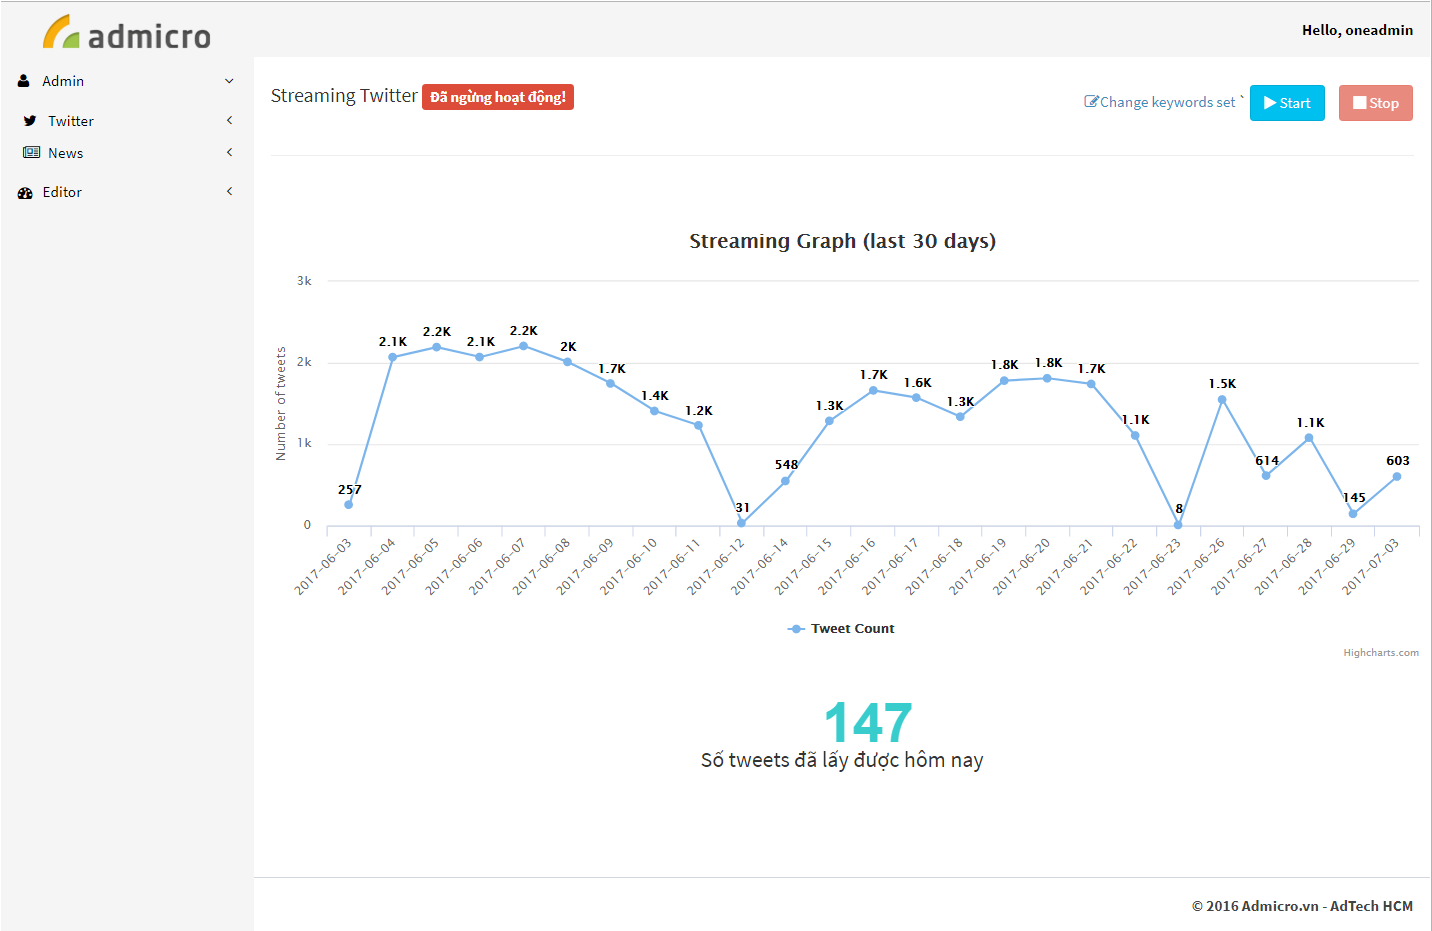
\includegraphics[width=1\linewidth]{Chapter3/Chapter3Figs/StreamingNonwide}
	\caption{Giao diện điều khiển thu thập dữ liệu Twitter}
	\label{fig:streaming}
\end{figure}

\begin{figure}[H]
	\centering
	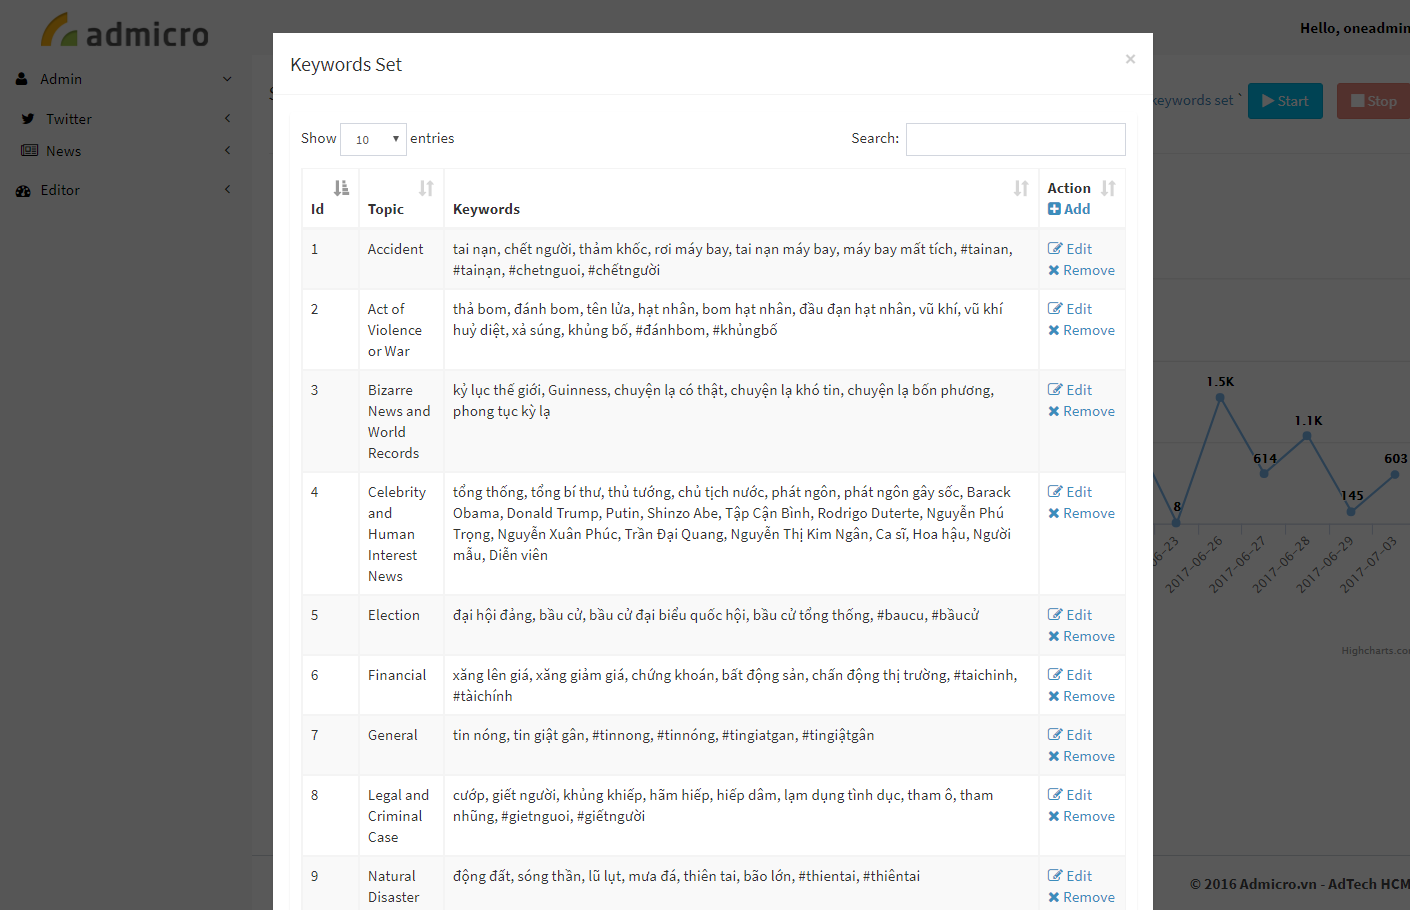
\includegraphics[width=0.96\linewidth]{Chapter3/Chapter3Figs/StreamingKeywords}
	\caption{Giao diện thêm xóa từ khóa để thu thập dữ liệu Twitter}
	\label{fig:streamingkeywords}
\end{figure}

\begin{figure}[H]
		\centering
	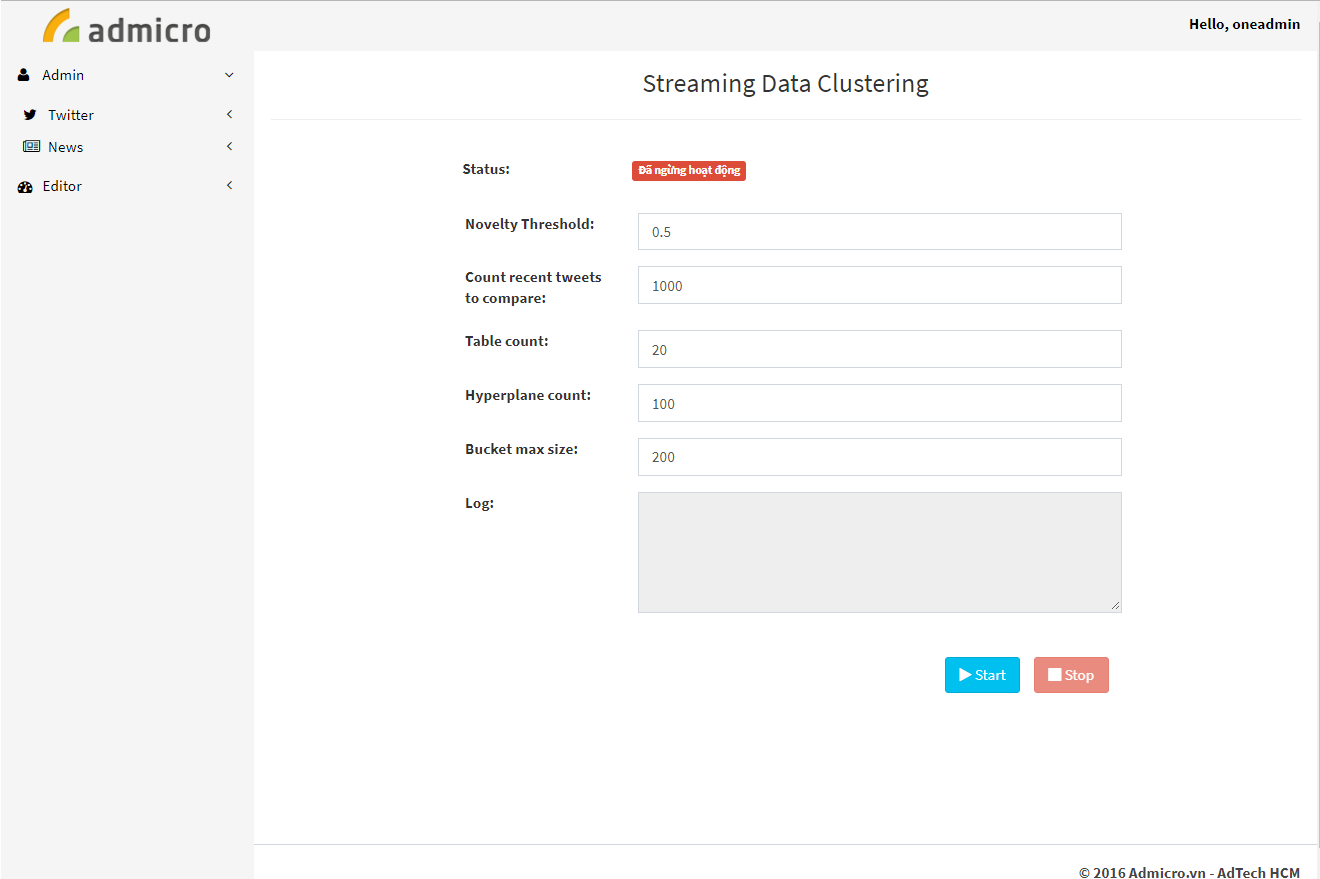
\includegraphics[width=0.96\linewidth]{Chapter3/Chapter3Figs/StartClustering}
	\caption{Giao diện điều khiển thuật toán phát hiện tin nóng}
	\label{fig:startclustering}
\end{figure}

\begin{figure}[H]
		\centering
	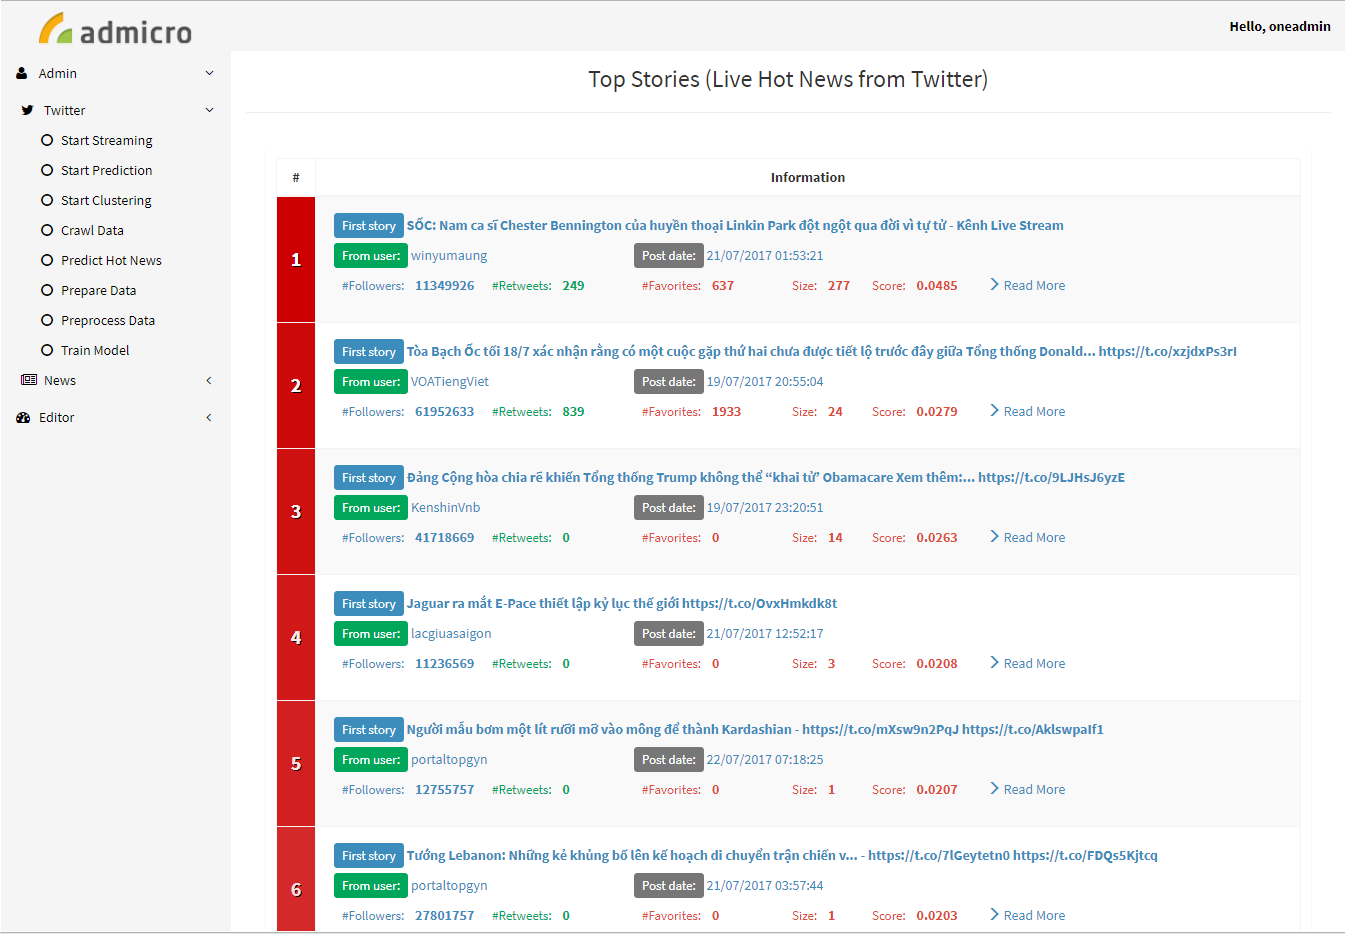
\includegraphics[width=0.96\linewidth]{Chapter3/Chapter3Figs/TopStories2}
	\caption{Giao diện hiển thị các cụm bài viết cho biên tập viên}
	\label{fig:topstories}
\end{figure}

\begin{figure}[H]
	\centering
	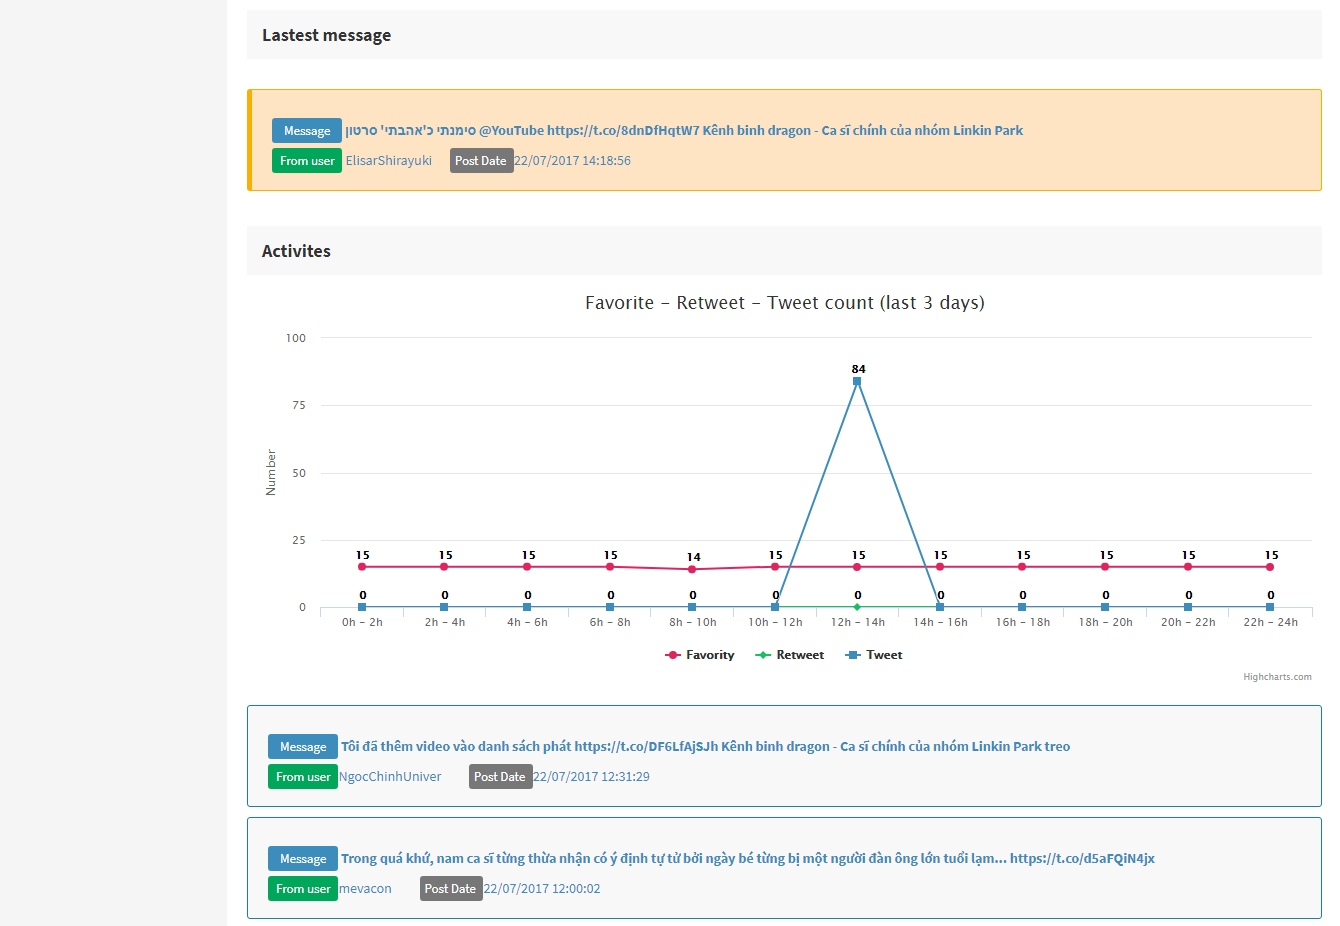
\includegraphics[width=0.96\linewidth]{Chapter3/Chapter3Figs/StoryDetails2}
	\caption{Chi tiết một cụm bài viết}
	\label{fig:storydetail}
\end{figure}

\section{Kết chương}
Chương này đã trình bày về các thành phần chính hệ thống, kiến trúc phân tầng, các hệ cơ sở dữ liệu được sử dụng và cách tổ chức, cùng một số kết quả cài đặt hệ thống.